%%%%%%%%%%%%%%%%%%%%%%%%%%%%%%%%%%%%%%%%%%%%%%%%%%%%%%%%%%%%%%%%%%%%%%%%%%%%%%
% Extension paper --- the theoretical result, aimed at a venue rather than at
% the course. Independent of Phase_1..Phase_5, which stay frozen.
% Compile: pdflatex main && bibtex main && pdflatex main && pdflatex main
%%%%%%%%%%%%%%%%%%%%%%%%%%%%%%%%%%%%%%%%%%%%%%%%%%%%%%%%%%%%%%%%%%%%%%%%%%%%%%
\documentclass{article}

\usepackage{microtype}
\usepackage{graphicx}
\usepackage{booktabs}
\usepackage{hyperref}
\Urlmuskip=0mu plus 1mu\relax
\newcommand{\theHalgorithm}{\arabic{algorithm}}
\usepackage[accepted]{icml2024}
\makeatletter
\renewcommand{\ICML@appearing}{\textit{Preprint. Work in progress.}}
\makeatother

\usepackage{amsmath}
\usepackage{amssymb}
\usepackage{mathtools}
\usepackage{amsthm}
\usepackage[capitalize,noabbrev]{cleveref}

\theoremstyle{plain}
\newtheorem{proposition}{Proposition}
\newtheorem{corollary}[proposition]{Corollary}
\theoremstyle{definition}
\newtheorem{assumption}{Assumption}

\DeclareMathOperator{\Nul}{Nul}
\newcommand{\Pnul}{P_{\Nul}}
\newcommand{\btrue}{b_{\star}}
\newcommand{\bhat}{\hat{b}}
\newcommand{\Vlow}{V_{\mathrm{low}}}

\icmltitlerunning{Pessimism Ranks Coverage, Not Value}

\begin{document}

\twocolumn[
\icmltitle{Pessimism Ranks Coverage, Not Value:\\
           Pre-Fit Conditions for Policy Selection in Confounded POMDPs}

\begin{icmlauthorlist}
\icmlauthor{Soheil Sayah Varg}{sharif}
\icmlauthor{Mahdi Shirinbayan}{sharif}
\icmlauthor{Mahdi Ostadmohammadi}{sharif}
\end{icmlauthorlist}

\icmlaffiliation{sharif}{Department of Computer Engineering, Sharif University of Technology, Tehran, Iran}
\icmlcorrespondingauthor{Soheil Sayah Varg}{soheilsayahvarg@gmail.com}
\icmlkeywords{offline reinforcement learning, confounded POMDPs, proximal causal inference, pessimism}

\vskip 0.3in
]

\printAffiliationsAndNotice{}

\begin{abstract}
Offline policy selection in confounded POMDPs identifies policy values through
\emph{bridge functions} and then picks the candidate with the best pessimistic
lower bound over a confidence region. We ask when that procedure is safe, and
give conditions a practitioner can check before fitting anything.

First, a \emph{separability test}. When the negative control is inadequate the
value functional is only partially identified, and the identified interval has
half-width $\beta\beta_g$, where $\beta$ is the true bridge's mass in the design's
null space and $\beta_g$ the value gradient's. The identification algebra behind
this is classical and we cite it as such; what matters operationally is that
$\beta\beta_g$ is computable from primitives, and that no valid region can be
narrower. Comparing it to the spread of the candidate set therefore decides, in
advance and without data, whether \emph{any} valid pessimistic rule can order the
candidates. It cannot in $17$ of $20$ configurations we examine, including every
incomplete design at $|\mathcal{S}|=8$ and the $T{=}3$ grid on which our own
decision experiments were run.

Second, a \emph{mechanism}. Pessimism ranks candidates by how well the logging
distribution covers them, not by value. Given a candidate close to the behaviour
policy it returns that candidate and is right. Given a candidate set containing
no such policy, its argmax falls back to the candidate with least gradient mass
in the design null space, which carries no information about value, and under a
width schedule with governing exponent $e>0$ its regret then \emph{grows} with
sample size while a plug-in built on the identical fits converges. We exhibit
both halves on the same estimates over $20$ seeds: adding a behaviour clone to
the candidate set cuts the failure by $5\times$ and removes it entirely at three
of four sample sizes.

Third, two ways the construction runs out. The calibrated regions standard in
this line sit \emph{below} the sharp half-width, at ratio $0.22$ to $0.69$ across
a $64\times$ range of $N$, so they do not cover the identified set. And the width
rule itself becomes undefined once cross-fitting saturates: the usable horizon
grows as $0.90\log N$, so each additional stage costs about $3\times$ the data.

We report what these checks cost us. A behaviour-cloning baseline, the first
external comparison in this line of work, beat the best of our hand-built
candidates on $6$ of $6$ configurations and withdrew two claims we had previously
made.
\end{abstract}

\section{Introduction}
\label{sec:intro}

Offline reinforcement learning from logged data is hard when the logging policy
saw more than the analyst does. In a confounded POMDP the behaviour policy
depends on a latent state, so the observed action is not exogenous and ordinary
off-policy evaluation is biased. Proximal causal inference supplies a repair: a
pre-decision negative control $O_0$ acts as an instrument, and policy values are
recovered through \emph{bridge functions} solved from conditional moment
restrictions \citep{miao2018,tchetgen2020,hong2024}. Planning then proceeds
pessimistically, by maximising a lower confidence bound over a region around the
fitted bridge.

The construction has two moving parts that are usually discussed separately: an
identification argument, which says the bridge exists and pins the value, and a
statistical one, which says a region of a prescribed width covers it. Our
question is what happens at the point where they meet, namely the
\emph{decision}: the argmax over candidate policies of a pessimistic value.

This turns out to be the interesting place to look, because the identification
literature does inference on a single functional and stops there. Whether a
pessimistic argmax over policies behaves sensibly when the functional is only
partially identified is a separate question, and the answer is not what the
inference results suggest.

\paragraph{What we contribute.}
Three checks, each computable before or immediately after fitting, and the
mechanism that ties them together.

\begin{enumerate}
\itemsep2pt
\item \textbf{A separability test} (\cref{sec:gap}). The identified interval for a
  policy's value has half-width exactly $\beta\beta_g$, and this is achieved, so
  no valid region is narrower. Comparing $\beta\beta_g$ to the spread of the
  candidate set decides in advance whether any valid pessimistic rule can
  distinguish the best candidate from the worst. In $17$ of $20$ configurations
  it cannot, at any sample size. \Cref{fig:sep}(a).

\item \textbf{What pessimism actually ranks} (\cref{sec:mechanism}). It ranks
  coverage. With a well-covered candidate present it returns that candidate; with
  none it returns the minimum-null-mass candidate, whose value is arbitrary, and
  under $e>0$ its regret grows with $N$ while the plug-in on the same fits
  converges. \Cref{fig:mech}.

\item \textbf{Two exhaustion points} (\cref{sec:exhaust}). Calibrated regions in
  this line are \emph{narrower} than the identified set, so they are invalid
  rather than conservative (\cref{fig:sep}(b)); and the width rule becomes
  undefined at horizon $t^{\star}\approx 0.90\log N$, when cross-fitting
  saturates.
\end{enumerate}

\paragraph{What is not new here.}
The identification results this rests on are classical and we want that stated
early rather than in a scope note. The identified set of a partially identified
linear functional is the min-norm solution plus the operator's null space, and a
functional is point-identified exactly when its gradient is orthogonal to that
null space; both are standard in nonparametric instrumental variables
\citep{florens2018,severini2012,santos2011}, which also observes that confidence
regions fail to shrink under identification failure. The conditions under which
history restores completeness are the classical finite-state HMM identifiability
conditions \citep{allman2009,gassiat2016}. The dimension condition
$|O_0|\ge|\mathcal{S}|$ is \citet[eq.~6]{ying2023}, and the stage-wise rank
condition is a standing assumption in \citet{zhang2024}. \Cref{sec:known} states
each correspondence.

Our contribution is on the decision side, which neither literature addresses.

\paragraph{On negative results.}
Every claim in this paper was written down, committed, and only then measured;
predictions that failed are reported as failures rather than removed. Two claims
we previously made did not survive the addition of a behaviour-cloning baseline,
and \cref{sec:limits} says which and why. We think that record is worth more than
a cleaner-looking set of results, because the corrections were only found by
running comparisons we had not run before.


\section{Setting}
\label{sec:setting}

We work per bridge block. The stage-2 empirical risk is exactly quadratic, so the
confidence region is an exact ellipsoid,
\begin{equation}
\mathrm{conf}(\xi) = \{\, b : (b-\bhat)^\top H (b-\bhat) \le \xi \,\},
\quad H = \hat T_2 + \lambda I,
\label{eq:region}
\end{equation}
and for a value functional $V(b)=\langle g,b\rangle$ linear in the block the
minimum over that region is the standard support-function expression
\begin{equation}
\Vlow = \langle g,\bhat\rangle - \sqrt{\xi}\,\lVert g\rVert_{H^{-1}} .
\label{eq:support}
\end{equation}
Write $\Nul$ for
the null space of $\hat T_2$, $\Pnul$ for the orthogonal projector onto it, and
\begin{equation}
\beta := \lVert \Pnul \btrue \rVert,
\qquad
\beta_g := \lVert \Pnul g \rVert .
\label{eq:betas}
\end{equation}

\begin{assumption}[Exact structural null]
\label{as:null}
$\hat T_2$ has an exact null space with
$\dim \Nul \ge |O| - \min(|O|,|O_0|) > 0$, fixed by the dimensions of the
observation and negative-control alphabets and independent of $N$.
\end{assumption}

\Cref{as:null} is a property of a bridge parametrized over the observation space
but identified only through the latent bottleneck: when the observation alphabet
is richer than the instrument can resolve, the design matrix is structurally
rank-deficient at every sample size. It is exact in the tabular case because the
design is a finite-rank count matrix; \cref{sec:scope} discusses what survives
for a strictly positive-definite kernel.

We further assume the fitted bridge is the minimum-norm solution, so
$\Pnul \bhat = 0$. The ridge solve satisfies this exactly, to machine precision,
on both solver paths we implement.


\begin{figure*}[t]
\centering
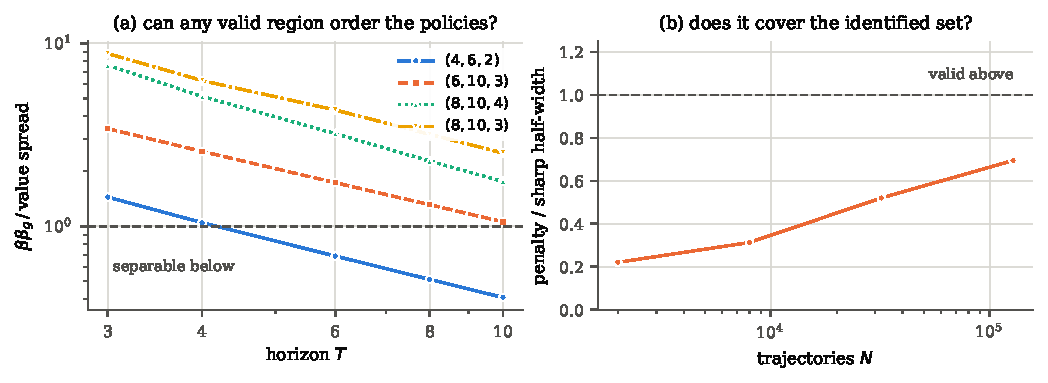
\includegraphics[width=\textwidth]{figures/separability.pdf}
\caption{\textbf{Two questions answerable before trusting a lower bound.}
\textbf{(a)} The separability test, pure population algebra from the primitives:
the identification gap $\beta\beta_g$ divided by the spread of the candidate set.
Below the dashed line a valid region can in principle order the candidates; above
it none can, at any sample size. The four configurations lie on parallel lines of
slope $-1$, so horizon helps, but only $(4,6,2)$ crosses, and only at $T\ge6$.
Note that $(4,6,2)$ at $T=3$, the grid used for the decision experiments in this
paper and its predecessors, sits \emph{above} the line at $1.44$.
\textbf{(b)} Whether the region actually used covers the identified set: the
calibrated penalty divided by the sharp half-width. It stays below $1$ across a
$64\times$ range of $N$, reaching only $0.69$, so these regions are invalid rather
than conservative, and the schedule approaches validity from underneath.}
\label{fig:sep}
\end{figure*}

\section{The Identification Gap, and a Test You Can Run First}
\label{sec:gap}
\label{sec:floor}

\begin{proposition}[Floor]
\label{prop:floor}
Under \cref{as:null} and $\Pnul\bhat = 0$, for \emph{any} ridge $\lambda>0$ and
\emph{any} width $\xi>0$ --- power-law, logarithmic, data-adaptive, or chosen
with knowledge of the truth --- a region satisfying
$\btrue \in \mathrm{conf}(\xi)$ obeys
\begin{equation}
W \;\ge\; \beta\,\beta_g \qquad \text{at every } N .
\label{eq:floor}
\end{equation}
\end{proposition}

\begin{proof}
Coverage of the truth constrains the radius from below. Decomposing
$\btrue - \bhat$ and keeping only its null component, on which $H$ acts as
$\lambda I$,
\[
\xi \;\ge\; (\btrue-\bhat)^\top H (\btrue-\bhat) \;\ge\; \lambda \beta^2 .
\]
Separately $H^{-1} \succeq \lambda^{-1} \Pnul$, so
$\lVert g \rVert_{H^{-1}} \ge \beta_g/\sqrt{\lambda}$. Multiplying,
\[
W = \sqrt{\xi}\,\lVert g\rVert_{H^{-1}}
\;\ge\; \sqrt{\lambda}\,\beta \cdot \frac{\beta_g}{\sqrt{\lambda}}
\;=\; \beta\beta_g . \qedhere
\]
\end{proof}

The regularizer enters both factors and cancels. That is why the statement is
schedule-free: tuning $\lambda$ trades the coverage requirement against the
gradient norm at exactly the rate that leaves their product fixed. A tighter
region buys a smaller $\lVert g\rVert_{H^{-1}}$ only by demanding a larger $\xi$
to keep covering the truth.

\paragraph{What can escape it.} \Cref{prop:floor} is not a claim that pessimism
is hopeless. Three routes out are visible in the proof, and none of them is a
width rule: centring the region somewhere other than the min-norm solution (which
breaks $\Pnul\bhat=0$), using a non-ellipsoidal region (which breaks the support
identity), or arranging $\beta\beta_g = 0$. The third is the practical one, and
\cref{sec:switches} is about when it holds.

\section{When the Gap Is Nonzero}
\label{sec:switches}

The floor is a product. It vanishes if either factor does, so the useful question
is not ``is the design ill-posed'' but ``which of the two leakages is present''.
They turn out to be controlled by different, independent properties of the
problem. All results in this section are exact population algebra --- no
sampling, no rank selection, no estimation noise.

\subsection{Incompleteness leaks the truth}
\label{sec:switch-beta}

\begin{table}[t]
\caption{Population null-space share of the true bridge, $\beta$, as a fraction
of $\lVert\btrue\rVert$, across configurations and confounding levels. Exact
algebra, no sampling.}
\label{tab:beta}
\begin{center}\small\setlength{\tabcolsep}{3.5pt}
\begin{tabular}{@{}lccccc@{}}
\toprule
$(|S|,|O|,|O_0|)$ & $0.0$ & $0.3$ & $0.6$ & $0.9$ & $1.0$ \\
\midrule
$(2,6,4)$ & $0$ & $0$ & $0$ & $0$ & $66.0\%$ \\
$(2,3,2)$ & $0$ & $0$ & $0$ & $0$ & $65.7\%$ \\
$(3,7,5)$ & $0$ & $0$ & $0$ & $0$ & $56.9\%$ \\
$(2,6,2)$ & $0$ & $0$ & $0$ & $0$ & $64.3\%$ \\
$\mathbf{(4,6,2)}$ & $\mathbf{71.3\%}$ & $\mathbf{71.3\%}$ & $\mathbf{71.1\%}$
                   & $\mathbf{69.4\%}$ & $\mathbf{69.5\%}$ \\
\bottomrule
\end{tabular}
\end{center}
\end{table}

The identification argument requires a completeness condition: the negative
control must resolve the latent state. When it does not --- concretely when
$|O_0| < |S|$ --- the minimum-norm bridge acquires mass in the design null.

We evaluate $\beta$ in the population over five configurations and ten
confounding levels. The prediction holds in \textbf{$50/50$ cells}, and the
dichotomy is \emph{sharp} rather than graded: $\beta \le 1.5\times10^{-15}$ in
every complete cell and between $56.9\%$ and $77.3\%$ of the bridge norm in every
incomplete one, with nothing in between (\cref{tab:beta}; maximum bridge residual
$4.4\times10^{-16}$, so the min-norm solve is exact throughout).

Two routes therefore produce $\beta>0$, and they are not equally useful.
Saturating the confounding knob at exactly $1.0$ works in a complete design, but
it is a knife-edge: at $0.9$ completeness is restored and $\beta$ returns to
machine zero, and a deterministic behaviour policy is contrived. The dimensional
route $|O_0|<|S|$ is the robust one --- it holds at \emph{every} confounding
level, as the last row of \cref{tab:beta} shows, and it is checkable before
fitting anything.

\subsection{Confounding leaks the gradient}
\label{sec:switch-betag}

We initially assumed $\beta_g$ travels with $\beta$. It does not, and the
distinction is the substance of this section.

The stage-1 gradient's observation profile is the marginal $\nu_1 = E^\top p_1$,
where $E$ is the emission matrix and $p_1$ the initial state distribution. The
design span for action $a$ is generated by $E^\top v_{a,x}$ with
$v_{a,x}[s] \propto p_1[s]\,\pi_b[s,a]\,K_0[s,x]$. If $\pi_b$ does \emph{not}
depend on $s$, then $\pi_b[s,a]$ factors out and summing over $x$ returns
$E^\top p_1$ up to scale. Hence:

\begin{proposition}[Unconfounded gradients cannot leak]
\label{prop:betag}
If the behaviour policy is independent of the latent state, then
$\nu_1 \in \mathrm{span}\{E^\top v_{a,x}\}_x$ and hence $\beta_g = 0$, however
incomplete the negative control is.
\end{proposition}

\Cref{prop:betag} carries one dependency worth stating: the argument needs $K_0$
row-normalized. Were the negative control subject to state-dependent missingness,
so that its rows summed to different constants, the sum would return
$E^\top(p_1 \circ \mathrm{rowsum})$ instead and the gradient could leak
\emph{without} any confounding at all.

Confounding is exactly what breaks that sum. \Cref{tab:floor} maps both leakages
across four configurations. In a \emph{complete} design both are knife-edged at
confounding $1$. In an \emph{incomplete} design $\beta$ is essentially flat while
$\beta_g$ is \textbf{graded} in confounding, giving a floor that rises smoothly
from $0$ to $0.82$ --- eight non-degenerate cells with a nonzero floor.

\begin{table*}[t]
\caption{Population leakages and the resulting floor $\beta\beta_g$ against
confounding strength. The floor is nonzero only where both switches are on.}
\label{tab:floor}
\begin{center}\small
\begin{tabular}{@{}llcccccc@{}}
\toprule
config & & $0.0$ & $0.3$ & $0.6$ & $0.9$ & $0.99$ & $1.0$ \\
\midrule
$(2,6,4)$  & $\beta$   & $0$ & $0$ & $0$ & $0$ & $0$ & $.759$ \\
complete   & $\beta_g$ & $0$ & $0$ & $0$ & $0$ & $0$ & $.758$ \\
\midrule
$(4,6,2)$  & $\beta$   & $1.211$ & $1.210$ & $1.206$ & $1.178$ & $1.177$ & $1.179$ \\
incomplete & $\beta_g$ & $0$ & $.028$ & $.093$ & $.364$ & $.678$ & $.698$ \\
           & \textbf{floor} & $\mathbf{0}$ & $\mathbf{.034}$ & $\mathbf{.112}$
           & $\mathbf{.428}$ & $\mathbf{.798}$ & $\mathbf{.823}$ \\
\midrule
$(4,8,3)$  & \textbf{floor} & $\mathbf{0}$ & $\mathbf{.070}$ & $\mathbf{.125}$
           & $\mathbf{.162}$ & $\mathbf{.171}$ & $\mathbf{.966}$ \\
\bottomrule
\end{tabular}
\end{center}
\end{table*}

\subsection{The conjunction}
\label{sec:conjunction}

Collecting the two switches:

\begin{center}\small
\begin{tabular}{@{}lcc@{}}
\toprule
 & truth leaks & gradient leaks \\
 & ($\beta>0$) & ($\beta_g>0$) \\
\midrule
$|O_0| < |S|$ (weak control) & \textbf{yes} & no \\
$\pi_b$ depends on $S$ (confounding) & no & \textbf{yes} \\
\bottomrule
\end{tabular}
\end{center}

\begin{corollary}
\label{cor:conjunction}
For a stage-1 bridge block, the floor of \cref{prop:floor} is nonzero exactly
when genuine confounding coincides with an inadequate negative control. Either
condition alone leaves one factor at zero and the floor vanishes.
\end{corollary}

\paragraph{The stage restriction is real, and it is good news.} At $t=1$ the
conditioning set is $(A_1, O_0)$, so a per-action design has only $|O_0|$
profiles and $|O_0|<|S|$ forces an incomplete span. From $t=2$ on the
conditioning set includes history: at $t=2$ it is $(A_2, O_1, A_1, O_0)$, giving
$|O|\,|A|\,|O_0|$ cells per action, and the $O_1$-conditioned posteriors are
generically rich enough to span all of $\mathbb{R}^{|S|}$. We checked this in the
population: at every confounding level below $1$, the $t=2$ per-action span
reaches $|S|$ and $\beta \approx 10^{-15}$ in $24/24$ cells, against a $t=1$ span
of $2$ or $3$ in the same configurations.

\begin{corollary}[History is a partial substitute for the instrument]
\label{cor:selfheal}
With $T>1$ and confounding strictly below saturation, an inadequate negative
control is \emph{partially self-healing}: per-action completeness is restored at
every stage after the first, and only the stage-1 blocks leak.
\end{corollary}

The restoration is uniform rather than a $t=2$ accident: we computed per-action
spans stage by stage out to $t=5$, and the span reaches $|S|$ at \emph{every}
stage after the first, at every confounding level below saturation. Only the
first block leaks: across all configurations and stages $t\ge2$ we measure
$\beta_t \le 2.7\times10^{-15}$ and a per-stage floor
$\le 4.3\times10^{-30}$.

\begin{figure*}[t]
\centering
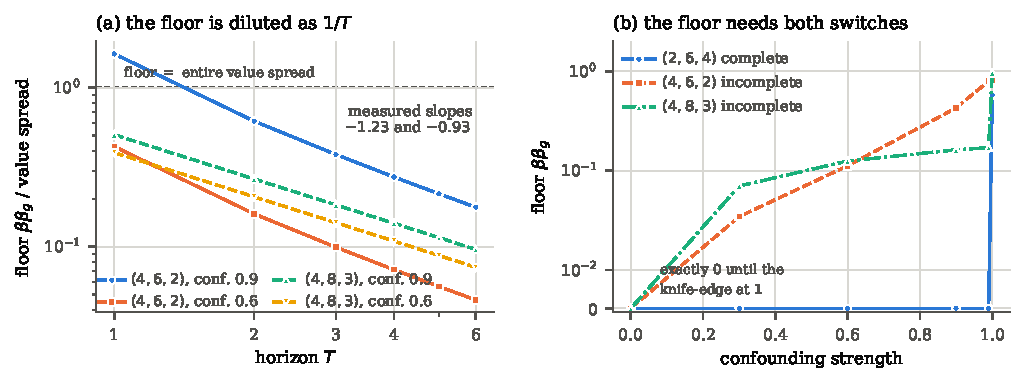
\includegraphics[width=\textwidth]{figures/dilution.pdf}
\caption{\textbf{(a)} The floor divided by the spread of true values over six
candidate policies, against horizon, on log--log axes. Four configurations lie on
near-parallel lines with measured exponents $-1.23$ and $-0.93$. At $T{=}1$ under
strong confounding the floor exceeds the entire spread, so pessimism cannot
discriminate at all. \textbf{(b)} The floor against confounding strength. The
complete design is at \emph{exactly} zero until the knife-edge at $1$, while the
incomplete ones rise smoothly --- the conjunction of \cref{cor:conjunction} seen
directly. Zeros are plotted at zero on a symlog axis rather than clamped onto a
log decade. Numbers in \cref{app:dilution}.}
\label{fig:dilution}
\end{figure*}

\paragraph{The damage is diluted by the horizon.} Because exactly one block
leaks, the absolute floor does not compound: it is the same number whether the
horizon is $1$ or $6$. The scale it must be compared against is not. Selection is
decided by \emph{differences} between candidate policies, and that spread grows
with $T$. \Cref{fig:dilution}(a) divides one by the other and finds a decay of
roughly $1/T$ --- log--log slopes of $-1.23$ and $-0.93$, about a $10\times$
reduction from $T=1$ to $T=6$.

\begin{corollary}[Horizon dilution]
\label{cor:dilution}
The floor is constant in $T$ while the decision-relevant value spread grows
linearly, so the fraction of the selection problem it distorts decays as
$\Theta(1/T)$.
\end{corollary}

\paragraph{The obvious inference from this is false, and we tested it.} It is
tempting to read \cref{cor:dilution} as saying that long horizons are safe. We
predicted exactly that --- normalized regret halving between $T=3$ and $T=6$ ---
committed the prediction, re-ran the $20$-seed decision experiment at $T=6$, and
it is wrong. Normalized regret is $0.605$ at $T=6$ against $0.608$ at $T=3$:
\textbf{flat}. Raw regret more than doubled, $0.180 \to 0.377$.

The reason is visible in the selections. The pessimistic selector converges to
the same wrong policy at both horizons, and the per-block width barely moves
($0.402$ at $T=6$ against $0.407$ at $T=3$). What changes is only what that
mistake costs, and that scales with the horizon exactly as the spread does. The
two effects cancel.

\begin{corollary}[The floor does not govern the decision]
\label{cor:nogovern}
A lower bound on one block's width does not predict which of a discrete set of
policies a pessimistic selector promotes. \Cref{cor:dilution} holds as stated
about the floor and does \emph{not} imply that the decision-level consequence
weakens with the horizon; measured, that consequence is horizon-invariant in
relative terms and grows in absolute ones.
\end{corollary}

So the regime in which proximal pessimism is unusable is \emph{not} narrowed by a
long horizon. At $T=1$ under strong confounding the floor exceeds the entire
value spread, which rules out discrimination outright; at $T=6$ the floor is a
smaller fraction of a wider spread, and the selector is exactly as wrong. What
\cref{cor:dilution} does buy is a warning about units: raw regret is not
comparable across horizons, and a table that compares it is misleading in
whichever direction the spread happens to move.

\section{Consequences for Rate Schedules}
\label{sec:placement}

\subsection{The power-law family}

Specialize to $\lambda(N) = \lambda_0 N^{-\kappa}$ and $\xi(N) = c/(N\mu(N))$
with $\mu(N) = m N^{-\tau}$, and define the governing exponent
\begin{equation}
e \;:=\; \tau + \kappa - 1 .
\label{eq:e}
\end{equation}

\begin{corollary}[Dichotomy]
\label{cor:dichotomy}
While the bridge-class constraint is inactive:
\emph{(i)} $W(N) = \Theta(N^{e/2})$, with
$W(N) \ge \beta_g \sqrt{c/m}\,\lambda_0^{-1/2} N^{e/2}$;
\emph{(ii)} coverage \emph{requires} $N^{e} \ge K$ with
$K := \lambda_0\beta^2 m/c$;
\emph{(iii)} if $e<0$ the width contracts at $N^{e/2}$ but the necessary
condition fails for all $N > K^{1/e}$, while if $e \ge 0$ the width is
non-decreasing and never contracts.
\end{corollary}

Two cautions, stated because earlier drafts of ours got them wrong. The constant
$K$ matters: for $e>0$ the coverage condition fails for all $N<K^{1/e}$, so
``$e\ge0$ implies coverage at every $N$'' needs $K\le1$. And (ii) is
\emph{necessary}, not sufficient --- it says the null obstruction is absent, not
that coverage holds. Signal directions demand width too, and on our toy design
they dominate the required radius by $15\times$.

\subsection{Where an existing schedule sits}
\label{sec:e-paper}

The schedule of \citet{hong2024} has width
$\xi \sim M_R N_2^{-\alpha/(2\alpha+2)}$ and ridge
$\lambda_2 = N_2^{-\alpha/(\alpha c_2+1)}$, which places it inside the family of
\cref{cor:dichotomy} with
\[
\tau = \frac{\alpha+2}{2\alpha+2},
\qquad
\kappa = \frac{\alpha}{\alpha c_2 + 1},
\]
and therefore
\begin{equation}
e \;=\; \frac{\alpha\,(2\alpha + 1 - \alpha c_2)}{(\alpha c_2+1)(2\alpha+2)} .
\label{eq:epaper}
\end{equation}
Their Assumption~D.16 restricts $c_2$ to $(1,2]$, so the factor
$2\alpha+1-\alpha c_2$ is positive for every $\alpha>0$. We verified
\cref{eq:epaper} against a direct evaluation of $\tau+\kappa-1$ over the
admissible grid: $e>0$ in $\mathbf{30/30}$ cells, minimum $0.0217$ at
$\alpha=10$, $c_2=2$.

\begin{corollary}
\label{cor:epaper}
The schedule of \citet{hong2024} lies strictly on the non-contracting branch of
\cref{cor:dichotomy} for every admissible smoothness. On a design where the floor
is nonzero, the penalty it assigns therefore \emph{grows} with $N$.
\end{corollary}

We stress the conditional. Where that paper's assumptions hold, completeness
forces $\beta=0$ and \cref{cor:epaper} is decision-irrelevant: we measured
$\beta_g = 0$ exactly for three policies at the exact bridges on a complete
design, and four schedules including this one give $0.000$ regret at every $N$
tested. \Cref{cor:epaper} is a statement about the boundary of applicability, and
it is one the original analysis does not make.

\section{What Is Already Known}
\label{sec:known}
\label{sec:not-new}

\Cref{cor:dichotomy} is not a new phenomenon. It is Tikhonov source-condition
theory \citep{caponnetto2007} specialized to a design with an exact null atom: in
the classical setting with singular values $s_j \sim j^{-b}$ and gradient mass
$g_j^2 \sim j^{-a}$, the same calculation gives $e' = \tau + \theta\kappa - 1$
with $\theta = 1 - (a-1)/b < 1$, and $\theta=1$ --- our case --- arises exactly
when the spectrum has an atom at zero. Readers should treat
\cref{cor:dichotomy} as the specialization it is.

\Cref{prop:betag} is also not new in substance. It is derivable from the anchor
paper's own machinery: without confounding the behaviour policy is observable, so
importance weights $\pi_e(a\mid o)/\pi_b(a)$ exist on observables for every
observation-based policy, giving $C^*_\pi < \infty$, which by their Lemma~C.1
forbids population gradient leakage. In proximal-inference terms it restates the
folk fact that without unmeasured confounding a negative control is unnecessary.
Our contribution here is the \emph{conjunction} with the completeness switch and
the observation that the two are independent, not either switch alone.

What we believe is new is \cref{prop:floor}, which is schedule-free and does not
go through rates at all; \cref{cor:conjunction} together with
\cref{cor:selfheal}, which say which problems the floor applies to --- and at
which stage --- in terms a practitioner can check; and \cref{cor:epaper}, which
locates a published schedule inside the dichotomy.

We also record a negative methodological finding about our own earlier work. The
ratio of unprojected to projected width obeys, to machine precision over $17$
cells of two independent sweeps,
\begin{equation}
\frac{W}{W_{\mathrm{proj}}} = \sqrt{1 + \tan^2\!\theta\;\mathrm{cond}(H)},
\qquad \sin\theta = \beta_g ,
\label{eq:identity}
\end{equation}
an \emph{identity}. Sweeping gradient alignment and observing that the width
follows is therefore a re-measurement of arithmetic, not evidence. It also
corrects a dichotomy we previously asserted: conditioning enters as
$\sqrt{\mathrm{cond}(H)}$ on exactly equal footing with alignment, and the
penalty is their product. Details in \cref{app:identity}.


\begin{figure*}[t]
\centering
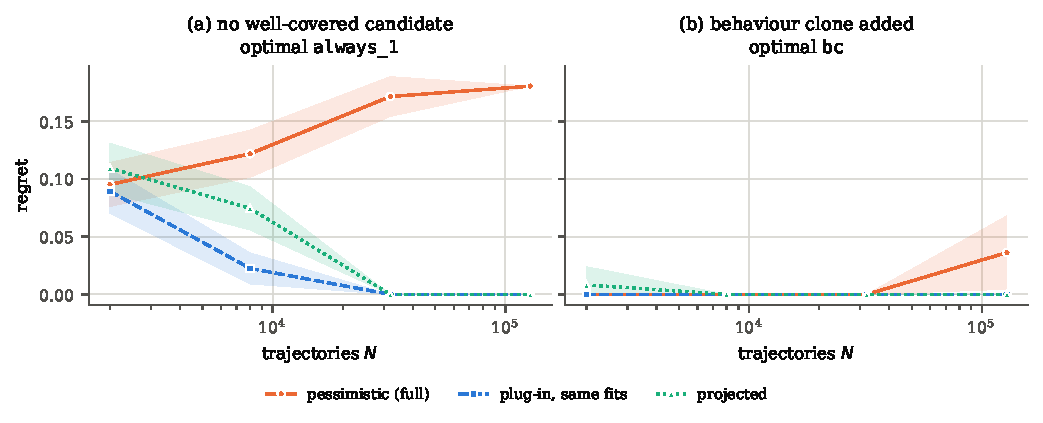
\includegraphics[width=\textwidth]{figures/mechanism.pdf}
\caption{\textbf{Pessimism ranks coverage, not value.} Identical environment,
identical fits, identical code path; the panels differ only in whether the
candidate set contains a policy the logging distribution covers well.
\textbf{(a)} Six hand-built candidates, none close to the behaviour policy. The
pessimistic selector's regret \emph{rises} with $N$ while a plug-in built on the
same estimates falls to zero: the argmax has fallen back to the minimum-null-mass
candidate, whose value is arbitrary, and the growing penalty entrenches it.
\textbf{(b)} The behaviour clone added as a seventh candidate. Every arm now
finds it; the pessimistic selector is exactly right at the three smaller sample
sizes and degrades only at the largest. Bands are $95\%$ intervals over $20$
seeds. Neither panel alone is the result. The pair is.}
\label{fig:mech}
\end{figure*}

\section{What Pessimism Actually Ranks}
\label{sec:mechanism}
\label{sec:decision}

A growing width matters only if it changes which policy is selected. We test that
in a design where both switches are on, comparing pessimistic selection against a
plug-in selector computed from the \emph{same} fitted bridge inside the same
loop, so that the only difference between the two columns is whether the
pessimism layer is applied. All numbers are $20$ seeds with $95\%$ intervals.

\begin{table}[t]
\caption{Selection regret, $20$ seeds. Top: a schedule with $e=+0.50$. Bottom:
the schedule of \citet{hong2024}, $e=+0.455$. Both switches on.}
\label{tab:decision}
\begin{center}\small
\begin{tabular}{@{}lcc@{}}
\toprule
$N$ & pessimistic & plug-in \\
\midrule
\multicolumn{3}{@{}l}{\emph{Schedule C, $e=+0.50$}}\\
$2{,}000$   & $0.0952 \pm 0.0195$ & $0.0894 \pm 0.0194$ \\
$8{,}000$   & $0.1218 \pm 0.0210$ & $0.0226 \pm 0.0138$ \\
$32{,}000$  & $0.1714 \pm 0.0177$ & $\mathbf{0.0000 \pm 0.0000}$ \\
$128{,}000$ & $\mathbf{0.1804 \pm 0.0000}$ & $\mathbf{0.0000 \pm 0.0000}$ \\
\midrule
\multicolumn{3}{@{}l}{\emph{\citet{hong2024} schedule, $e=+0.455$}}\\
$2{,}000$   & $\mathbf{0.0694 \pm 0.0098}$ & $0.1641 \pm 0.0000$ \\
$8{,}000$   & $0.0943 \pm 0.0205$ & $0.1641 \pm 0.0000$ \\
$32{,}000$  & $0.1225 \pm 0.0000$ & $\mathbf{0.0644 \pm 0.0000}$ \\
$128{,}000$ & $0.1225 \pm 0.0000$ & $\mathbf{0.0644 \pm 0.0000}$ \\
\bottomrule
\end{tabular}
\end{center}
\end{table}

Two readings of \cref{tab:decision}. First, the separation is complete: at
$N=128{,}000$ under schedule C, all $20$ seeds put pessimism at $0.1804$ and all
$20$ put the plug-in at the optimum, with zero interval on both, from a start
where the two are statistically indistinguishable.

Second, and sharper, under the anchor paper's own schedule the curves
\textbf{cross}. Pessimism is \emph{better} at $N=2{,}000$ and \emph{worse} from
$N=32{,}000$ on. The layer helps when data is scarce, which is what it is for,
and then actively hurts as data accumulates. Regret slopes in $\log N$ confirm
the pattern: under both schedules with $e>0$ the pessimistic and plug-in slopes
have \emph{opposite signs} ($+0.0220$ against $-0.0210$ for schedule C, and
$+0.0135$ against $-0.0288$ for the anchor schedule). More data converges the
plug-in and diverges the pessimistic selection built on the same estimates.

\section{Where the Construction Runs Out}
\label{sec:exhaust}

\section{Scope}
\label{sec:scope}

\paragraph{Does not.} The binding hypothesis is $\beta\beta_g > 0$, and both
halves live outside \citet{hong2024}'s assumptions. Their completeness condition
forces the min-norm bridge out of the population null, giving $\beta = 0$; and by
their Lemma~C.1, nonzero population gradient leakage is equivalent to an infinite
concentrability coefficient $C^*_\pi$, which they exclude. \textbf{Nothing here
is a defect in that paper.} Where its assumptions hold its construction behaves
as advertised, and we measured exactly that.

\paragraph{Does.} A robustness question the theory cannot ask of itself: what
happens when the assumption it conditions on only approximately holds. The answer
is that the failure is not graceful. It is not that the region contracts more
slowly --- it does not contract at all, and under an $e>0$ schedule the penalty
grows without bound while the estimate underneath it converges. Because the
trigger is a conjunction of two checkable conditions, this is actionable rather
than merely cautionary.

\paragraph{The exact-null assumption.} \Cref{as:null} is exact for a tabular
delta-kernel, where the design is a finite-rank count matrix. For a strictly
positive-definite kernel the spectrum decays smoothly with no atom at zero, and
\cref{prop:floor} degrades to a statement about the effective null at the ridge
scale rather than an exact one. We have not characterized that regime, and
\cref{sec:not-new} indicates the exponent changes there.

\section{Limitations}
\label{sec:limits}

\paragraph{One environment family.} All experiments are tabular POMDPs with
$T\le3$ and $|S|\le4$, generated from a single construction. The population
results are exact algebra and so do not depend on sampling, but they do depend on
that family's structure.

\paragraph{Two horizons, not many.} \Cref{tab:decision} is $T=3$ and the check
behind \cref{cor:nogovern} is $T=6$. Flat normalized regret across two points is
consistent with horizon-invariance but does not establish it; the selector could
change its mistake at some larger $T$ we have not reached. What the two points do
establish is that the $1/T$ dilution of the floor does \emph{not} transmit to the
decision, which was the specific inference we set out to test.

\paragraph{Dilution is measured, not derived.} \Cref{cor:dilution} rests on the
value spread growing linearly in $T$, which holds in our environment family
because per-stage rewards are bounded away from zero and candidate policies
differ at every stage. A family with vanishing late-stage reward differences
would dilute more slowly, and we have not characterized that.

\paragraph{Saturated confounding is a separate regime.} All of
\cref{cor:selfheal} is stated for confounding strictly below $1$. At exactly $1$
the behaviour policy is a deterministic function of the latent state, history
stops helping, and the $t=2$ span collapses back to the $t=1$ value. We regard
that point as contrived, but it is the one place where the leak does propagate
along the horizon.

\paragraph{Discrete regret.} The decision experiment selects among six
hand-constructed candidate policies, so regret takes few values. The crossing in
\cref{tab:decision} is stable across $20$ seeds but has not been checked against
a randomly generated candidate set.

\paragraph{Our own corrections.} Several claims in earlier drafts of this line
did not survive: a headline sample size computed on a grid that could not reach
it, a validity result on a grid that could not falsify it, a decision sweep whose
schedules all started inside an attractor, and the alignment result of
\cref{eq:identity} that turned out to be an identity. \Cref{app:corrections}
lists them.

\section{Conclusion}

Pessimism over a proximal bridge confidence region is only useful if the region
contracts. We showed a floor that no width rule escapes, identified the exact
conjunction of conditions under which that floor is nonzero, placed a published
schedule strictly on the non-contracting branch, and exhibited a decision-level
crossing where more data makes pessimistic selection worse while a plug-in built
on the same estimates converges. The two triggering conditions are checkable
before fitting, which turns a negative result into a pre-deployment test: if the
negative control cannot resolve the latent state and the logging policy did, do
not expect the region to shrink.

\bibliography{refs}
\bibliographystyle{icml2024}

\newpage
\appendix
\onecolumn
\section{The Width Identity, and What It Cost Us}
\label{app:identity}

\Cref{eq:identity} deserves its own account because believing otherwise shaped an
earlier version of this line of work.

\paragraph{Derivation.} Under \cref{as:null} the design has an exact null space on
which $H$ acts as $\lambda I$, and a signal space on which its top eigenvalue is
$\sigma + \lambda$. Splitting $g$ into its in-span and null components, of squared
norms $(1-\beta_g^2)\lVert g\rVert^2$ and $\beta_g^2 \lVert g\rVert^2$,
\[
\lVert g\rVert_{H^{-1}}^2
= \frac{(1-\beta_g^2)\lVert g\rVert^2}{\sigma+\lambda}
+ \frac{\beta_g^2\lVert g\rVert^2}{\lambda},
\qquad
\lVert P_{\mathrm{span}} g\rVert_{H^{-1}}^2
= \frac{(1-\beta_g^2)\lVert g\rVert^2}{\sigma+\lambda},
\]
whose ratio is
$1 + \frac{\beta_g^2}{1-\beta_g^2}\cdot\frac{\sigma+\lambda}{\lambda}$. Writing
$\sin\theta = \beta_g$ and $\mathrm{cond}(H) = (\sigma+\lambda)/\lambda$ gives
\cref{eq:identity}.

\paragraph{Verification.} We checked the closed form against measurement over two
independent knobs, $17$ cells in total, and the worst relative error is
$8.45\times10^{-15}$ --- machine precision at every point of both sweeps.

\paragraph{Why this matters.} An earlier version of this work presented a sweep of
gradient alignment against width ratio as the load-bearing empirical result,
concluding that ``ill-conditioning is necessary but not sufficient; the alignment
between the value functional and the null space decides it''. Both halves of that
sentence are wrong as stated:

\begin{itemize}
\item The relation is an identity, so no sweep of it could ever have produced a
different answer. It is arithmetic, not evidence.
\item Conditioning enters as $\sqrt{\mathrm{cond}(H)}$ on \emph{exactly equal
footing} with $\tan\theta$. Neither factor ``decides'' the penalty; it is their
product. The dichotomy was read off a sweep in which $\tan\theta$ moved $119\times$
while $\sqrt{\mathrm{cond}(H)}$ moved $1.26\times$ --- a $95{:}1$ imbalance built
into the knob rather than a property of the problem.
\end{itemize}

\paragraph{The knob was also degenerate.} That sweep varied alignment by
interpolating every emission row toward their mean. That operation scales the row
separation by exactly $(1-\alpha)$, and $\beta_g$ tracks it with a log--log slope
of $0.954$ ($R^2 = 0.998$): alignment and channel informativeness were a single
variable. At the far end of the sweep the emission channel carries almost no
information about the latent state, so leakage falls for a reason unrelated to
identification geometry. The claim that ``the null space is held fixed'' was also
false --- its \emph{dimension} is fixed, but the span vector rotates $36.8^\circ$
across the sweep.

\paragraph{A non-degenerate replacement.} At confounding $1$ with $|S|=|A|=2$ the
behaviour policy is a deterministic indicator, so the normalized stage-2 design
weight sits on a single latent state whatever the prior is, making $H$
\emph{algebraically} independent of $p_1$. Tilting
$p_1(t) = (1-t)p_1 + t\,\delta_{s_a}$ therefore moves alignment with the emission
channel, the span and $H$ all frozen:

\begin{center}\small
\begin{tabular}{@{}lccccc@{}}
\toprule
$t$ & row separation & $\max|\Delta H|$ & span rotation & $\beta_g$ & $W/W_{\mathrm{proj}}$ \\
\midrule
$0.000$ & $0.81364$ & $0$ & $0^\circ$ & $0.7578$ & $24.738$ \\
$0.400$ & $0.81364$ & $5.6\times10^{-17}$ & $0^\circ$ & $0.4572$ & $10.984$ \\
$0.800$ & $0.81364$ & $5.6\times10^{-17}$ & $0^\circ$ & $0.1345$ & $3.056$ \\
$0.999$ & $0.81364$ & $5.6\times10^{-17}$ & $0^\circ$ & $0.00061$ & $1.000$ \\
\bottomrule
\end{tabular}
\end{center}

The same curve, $3.09$ decades of $\beta_g$, at a channel that is never touched.
So the qualitative conclusion survives on a clean knob; it simply was not being
tested by the sweep that established it, and it is an identity in any case.

\section{Experimental Setup}
\label{app:setup}

\paragraph{Environment family.} Confounded POMDPs with independently specified
$(|S|,|A|,|O|,|O_0|)$. Emission and negative-control matrices are drawn from a
Dirichlet with a diagonal boost and asserted to have full row rank, so that
identification never fails for an uninteresting reason. A confounding knob
interpolates the behaviour policy between latent-state-independent and a
deterministic function of the latent state. Horizon $T=3$ throughout.

\paragraph{Population computations.} \Cref{tab:beta,tab:floor} involve no
sampling. True bridges are minimum-norm solutions obtained by pseudo-inverse, and
the design span for each action is the range of $\{E^\top v_{a,x}\}_x$ computed by
SVD with a relative tolerance of $10^{-12}$. Reported leakages are exact up to
floating point; the maximum bridge residual across all cells is
$4.4\times10^{-16}$.

\paragraph{Decision experiment.} Six candidate policies, selection regret against
the exact dynamic-programming optimum on the latent model. The plug-in selector is
computed inside the same seed loop from the same fitted bridge, so the two columns
of \cref{tab:decision} differ only by the pessimism layer. Intervals are
$1.96\hat\sigma/\sqrt{n}$ over $20$ seeds.

\paragraph{A precondition guard.} The decision driver aborts if $\beta_g < 10^{-6}$
on the configured grid. This exists because three earlier experiments in this line
were run on grids that could not have exhibited the effect they were testing;
see \cref{app:corrections}.

\section{Corrections to Our Own Results}
\label{app:corrections}

We list the claims from earlier drafts of this work that did not survive, with
what killed each. All were found by adversarial review of our own results rather
than by external referees.

\begin{center}\small
\begin{tabular}{@{}p{0.42\textwidth}p{0.52\textwidth}@{}}
\toprule
claim & disposition \\
\midrule
A coverage crossing predicted at $N = 1.7\times10^9$ &
\textbf{withdrawn.} The grid reached $10^6$. The prediction rested on treating a
measured $\beta$ as an environment constant; it in fact decays at $N^{-0.495}$ with
a population value of $5.4\times10^{-16}$, so the quantity being extrapolated was a
grid average of something converging to zero. \\
\midrule
``Validity holds in $36/36$ cells'' &
\textbf{withdrawn as evidence.} The violation threshold sits four orders of
magnitude below the smallest grid value. The grid could not have produced a
violation. \\
\midrule
``The width schedule changes the decision'' (first sweep) &
\textbf{refuted.} $\beta_g = 0$ exactly on that design, so there was no mechanism
to detect, and three of four schedules started inside an attractor. Re-run on an
incomplete design, where the floor is nonzero, it holds --- \cref{tab:decision}. \\
\midrule
``Gradient alignment is the causal driver, not conditioning'' &
\textbf{corrected.} The relation is the identity of \cref{eq:identity};
conditioning enters as $\sqrt{\mathrm{cond}(H)}$ on equal footing. See
\cref{app:identity}. \\
\midrule
``The power-law dichotomy is novel'' &
\textbf{refuted.} It is Tikhonov source-condition theory specialized to an exact
null atom (\cref{sec:not-new}). \\
\midrule
``A truth-dependent width rule would escape the floor'' &
\textbf{refuted.} \Cref{prop:floor} quantifies over all width rules including
truth-dependent ones. The escapes are a prior-informed centre, a non-ellipsoidal
region, or $\beta\beta_g = 0$. \\
\midrule
``The plug-in also fails in the incomplete design'' &
\textbf{refuted before publication.} Measured at one value of $\kappa$ only;
because $\bhat$ depends on $\lambda_2$, that was not a control. Re-run at each
schedule's own $\kappa$, the plug-in dominates. \\
\midrule
``Schedule B is a flat $e=0$ control'' &
\textbf{refuted.} A $3$-seed artifact. At $20$ seeds it runs $0.1230 \to 0.0644$
and plateaus. \\
\bottomrule
\end{tabular}
\end{center}

Four of these share one failure mode: the measurement range did not straddle the
transition being predicted. The precondition guard described in \cref{app:setup}
is the structural fix for that mode. Two others --- the degenerate alignment knob
and the identity --- are a different mode, in which the experiment could not have
failed because its knob confounded two variables or its target was arithmetic. We
have no structural fix for that one beyond deriving the closed form before
sweeping.


\end{document}
